\subsection{Finanzierung und wirtschaftliche Machbarkeit}\label{labelWirtMach}
%Gesamtplan 3-5 Jahre

Für die Berechnung unserer Finanzierung und der wirtschaftlichen Machbarkeit werden folgende Annahmen getroffen:

Als einzelne Kostenpositionen erwarten wir folgende Posten:
\begin{itemize}
\item Fixkosten
 \begin{itemize}
\item Serverkosten
\item Personalkosten
\item Büromiete
\item Kredittilgungen
 \end{itemize}
\item variable Kosten
\begin{itemize}
\item Marketingkosten
\item Entwicklungskosten
\item Transaktionsgebühren
\item Kreditzinsen
\item Bürobedarf/Sonstiges
\end{itemize}
\end{itemize}

Die Kosten für die Server ergeben sich aus den Betrachtungen im Kapitel \ref{labelTechMach}. Die vermuteten Kosten für das Büro sind dem aktuellen Hamburger Mietspiegel entnommen. Die Personalkosten verteilen sich auf die fünf Mitglieder dieses Unternehmens. Der für die Finanzierung benötigte Kredit erzeugt mit Zinsen und Tilgungen weitere Kosten.\\
Um die Kunden gewinnen zu können entstehen uns Kosten, die unter Marketingkosten zusammengefasst werden. Diese werden im laufe der Zeit abnehmen, wenn unser Bekanntheitsgrad ansteigt.\\
Die benötigte Software zur Zahlungsabwicklung mit den Kunden wird von uns selber entwickelt. Die veranschlagten Kosten sind unter dem Punkt Entwicklungskosten berücksichtigt. Die Entwicklungskosten werden im Laufe der Zeit abnehmen und werden um Wartungskosten ergänzt.\\
Weitere Kosten sind im Punkt Bürobedarf/Sonstiges zusammengefasst und können nur grob geschätzt werden.

Wie in Kapitel \ref{labelMarktuntersuchung} beschrieben, existieren diverse Spieleanbieter am Markt, die jeweils einen hohen Jahresumsatz erzielen. \\
Wir wollen mit unsren Kunden eine langfristige Geschäftsbeziehung eingehen. Wir setzen dabei darauf, dass wir nur einige wenige Kunden benötigen. Durch diese wenigen Kunden können wir aber hohe Umsätze erzielen.

Die Strategie, die wir bei der Kundengewinnung verfolgen, ist, dass wir zu Anfang mit einem Kunden starten und dann nach und nach weitere Kunden gewinnen. 

\subsubsection*{Gewinn und Verlustrechnung}
%24 auf monatlicher Basis, danach jährlich

\begin{figure}[htbp]
	\centering
	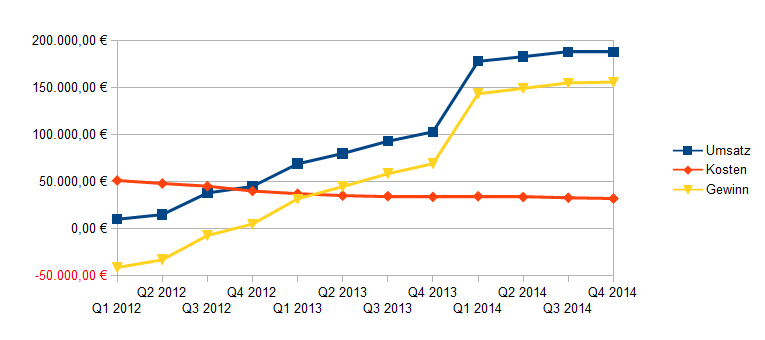
\includegraphics[width=1\textwidth]{GuV.png} 
	\caption{GuV}
	\label{picGuV}
\end{figure}

Die zu erwartenden Kosten betragen pro Quartal im Schnitt ca{.} 40.000,- Euro in den ersten 3 Jahren. Um Kostendecken arbeiten zu können müssen wir diesen Betrag über die Transaktionsgebühren wieder einholen. Wenn wir einen Anteil von 5\% an den Geldtransaktionen für uns einbehalten, dann müssen pro Quartal 800.000,- Euro bei den Kunden umgesetzt werden. 

Wie in Kapitel \ref{labelMarktuntersuchung} dargestellt, sind das sehr vorsichtige Berechnungen. Es ist davon auszugehen, dass der Umsatz bei den Kunden höher liegen wird. Dadurch können wir einerseits unsere eigenen Umsätze erhöhen und Gewinne einfahren, andererseits aber auch den prozentualen an den Kundenumsätzen verringern, was uns einen Vorteil bei Vertragsverhandlungen mit den Kunden einbringt.

\subsubsection*{Liquiditätsrechnung}
%24 auf monatlicher Basis, danach jährlich
\begin{figure}[htbp]
	\centering
	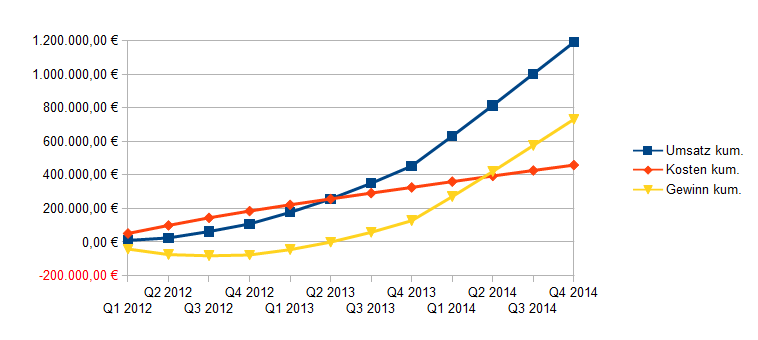
\includegraphics[width=1\textwidth]{GuVkummuliert.png}
	\caption{GuV kumuliert}
	\label{picGuVkum}
\end{figure}

Der Break-Even Punkt wird im vierten Quartal 2012 überschritten. Bis zum vorhergehenden Quartal addieren sich die Verluste auf ca{.} 82.000,- Euro (s. Abbildung \ref{picGuVkum}). Dieser Betrag wird mindestens benötigt, um die zu erwartenden Kosten zu decken.\\
Die Deckung der Kosten wird durch eine Bankfinanzierung geschehen. Dazu nehmen wir einen Kredit in Höhe von 90.000,- Euro mit einer Laufzeit von 4 Jahren und einem Zinssatz in Höhe von 5\%. Die monatlichen Tilgungsraten betragen 1.875,- Euro. Die Kosten sind in den übrigen Berechnungen bereits enthalten.
